\section{舞踊分類ネットワーク}

\subsection{モデル概要}
入力された動画を[優美なダンス,普通のダンス,その他の動作]に分類するために,
\begin{enumerate}
  \item 動画を下記で説明する二値化手法で編集する.
  \item 二値データと,それに対応するピクセル番号を畳み込む.
  \item 二つのデータを足し合わせる.
  \item Transformer Encoderに通した後,全結合し,Softmaxにかける.
\end{enumerate}
のようにネットワーク内で計算した.
最適化アルゴリズムにAdam\cite{adam},損失関数に交差エントロピー誤差(\ref{entropy})を使用した.
\begin{equation}
  H(p, q) = -\sum_{i}p_i\log q_i
  \label{entropy}
\end{equation}

\subsection{使用する動画データ}
\begin{table}[b]
  \begin{center}
    \begin{tabular}{|c|c|c|} \hline
      \ & 学習用 & 推論用 \\ \hline
      優美なダンス
        & \cite{jpn}\cite{china}\cite{ballet}\cite{thai}\cite{jpn2}
        & \cite{balletgroup}\cite{jpngroup}\cite{chinagroup}\cite{belly}
      \\ \hline
      普通のダンス
        & \cite{ariana}\cite{kadokawa}\cite{bts}\cite{manolo}\cite{aito}
        & \cite{btsgroup}\cite{arashi}\cite{hyoga}\cite{legit}
      \\ \hline
      その他の動作
        & \cite{radio}\cite{posing}\cite{boxing}\cite{running}\cite{shinkokyu}\cite{leaves}
        & \cite{radio2}
      \\ \hline
    \end{tabular}
  \end{center}
  \caption{使用した動画データ}
  \label{video_data}
\end{table}

動画は表\ref{video_data}を使用した.優美な動画の選定方法は,youtubeで優美,美しいなどの
キーワードで検索し,再生回数の多く,視聴した時に優美であると感じたものを使用した.
一つの国,舞踊の種類では目的である網羅的な学習を達成できないため,古今東西の舞踊を使用した.
普通のダンスでは同じようにダンスなどのキーワードを持ち,再生回数が多く,
視聴した時にダンスであると感じたものを使用した.その他の動作はランニングや体操など,
日常的な動作を使用した.再生回数が多いものを使用する理由は,その舞踊のエキスパートの動作を
できるだけ使用したかったからである.再生回数が多いということは,それだけ不特定多数から
注目を浴びている,感動を与えていると考えられ,その動作の熟練者である可能性が高いと考えた.

\begin{figure}[t]
  \begin{center}
    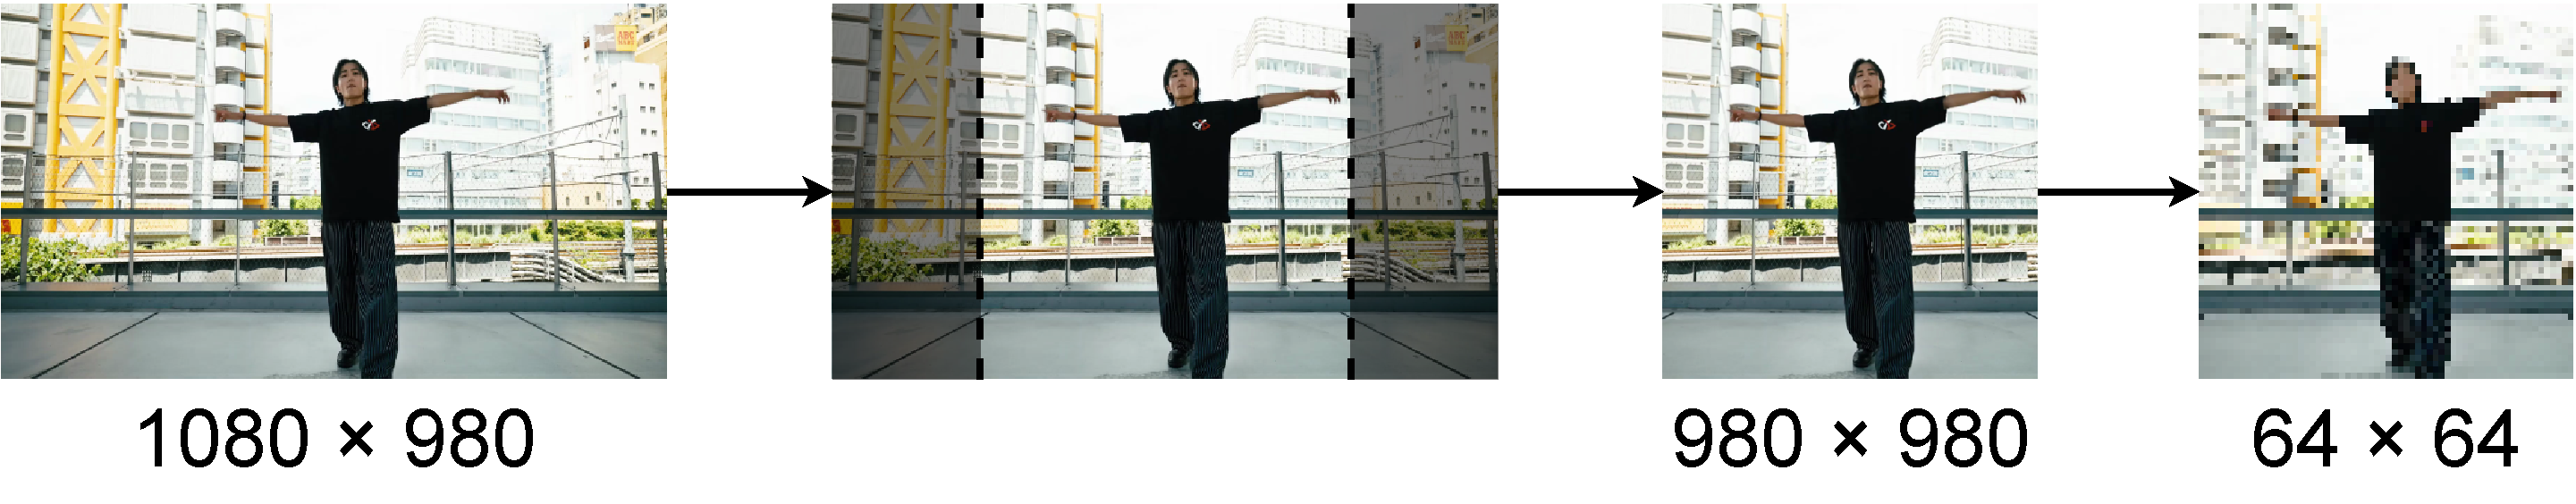
\includegraphics[width=120mm]{images/chart/resize.pdf}
  \end{center}
  \caption{動画の縮小例}
  \label{resize}
\end{figure}

動画の編集方法は,動画サイズを均一にするために図\ref{resize}のように縦横64ピクセルに縮小した.
縦横短い方を基準に長い方の両端を切り出し,OpenCVのresize\cite{resize}にかけた.
畳み込みでは正方形のフィルタを用いるため,動画サイズを正方形にする必要があった.
動画を確認した結果,64ピクセルが動作が確認できる最も小さなサイズであった.

次に,図\ref{binary}のように動画を二値化した.
グレースケール化した動画の1フレームごとの画像全体の平均をとった.
その平均より値の低いピクセルを255,高いピクセルを0にした.人体や服の色は
背景色より暗いことが多かったのでここではソフトに二値化した.

最後に図\ref{choice}のように白画素の制限を行なった.
先ほど二値化した動画の1ピクセルのフレーム長の配列を取り出した.
その配列の平均を取り,255/4に近い順で500画素まで採用した.
対象が黒画素であった場合はカウントしない.
閾値255/4はいくつか動画に制限処理を行なった中で,
多くの動画に対して,最も効果的に人体の輪郭を得ることができたため,このような値を用いた.

検証段階として,動画データをそのままネットワークにかけて学習した結果,精度が
ほとんど取れなかったので,動画データの統一が効果的ではないかと考えた.
二値に限定し,各ピクセル,動画全体のデータを均一にすることで学習の効率を高めることを試みた.

\begin{figure}[b]
  \begin{center}
    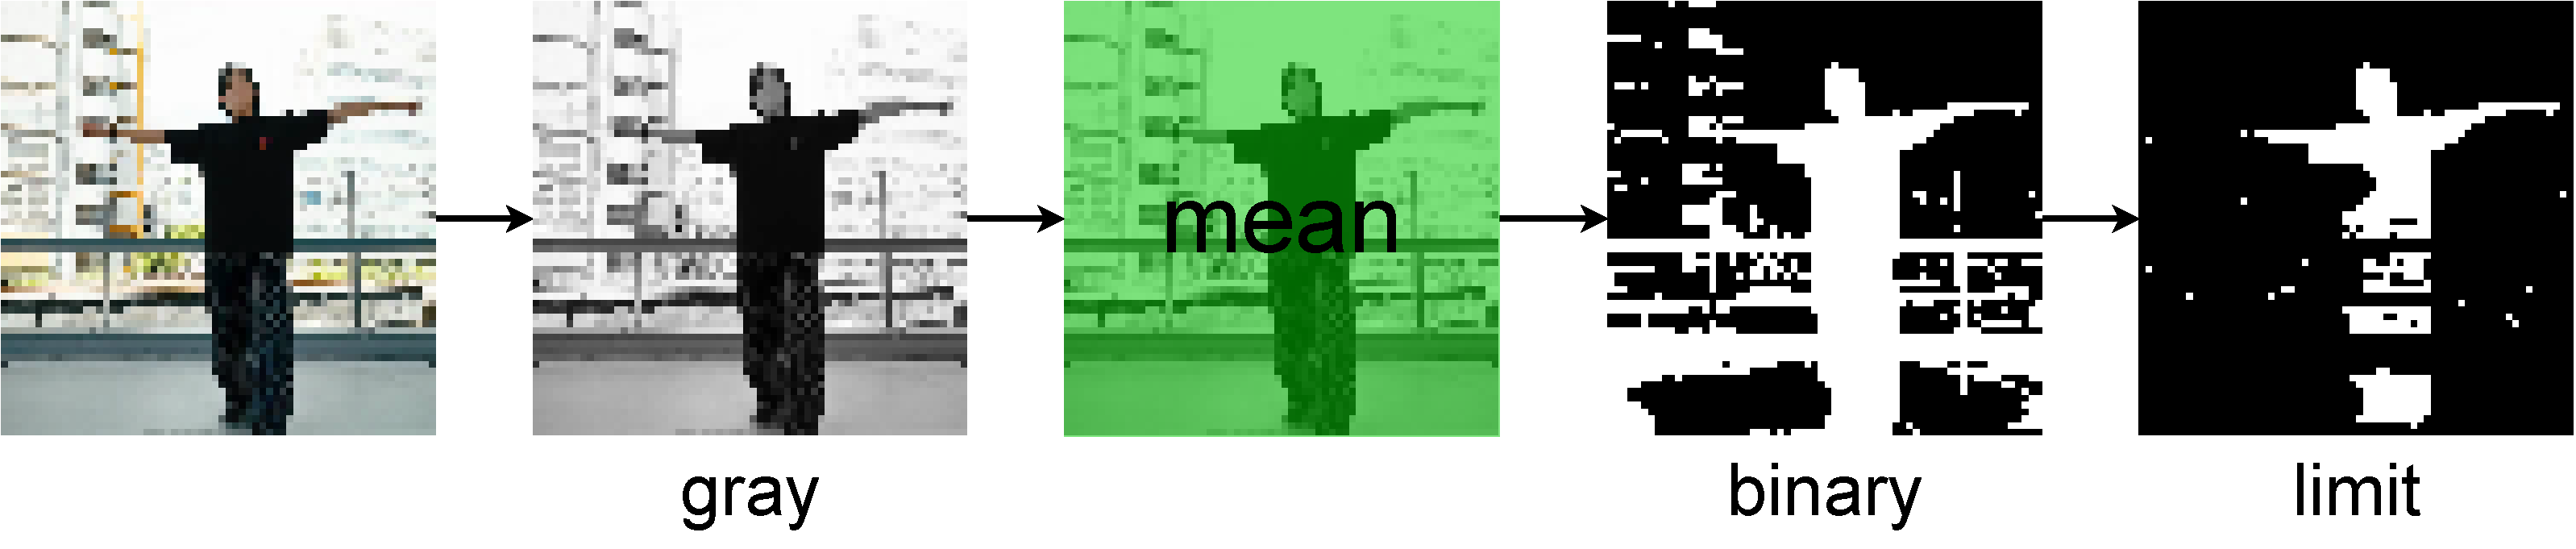
\includegraphics[width=120mm]{images/chart/binary.pdf}
  \end{center}
  \caption{動画の二値化例}
  \label{binary}
\end{figure}
\clearpage

\begin{figure}[t]
  \begin{center}
    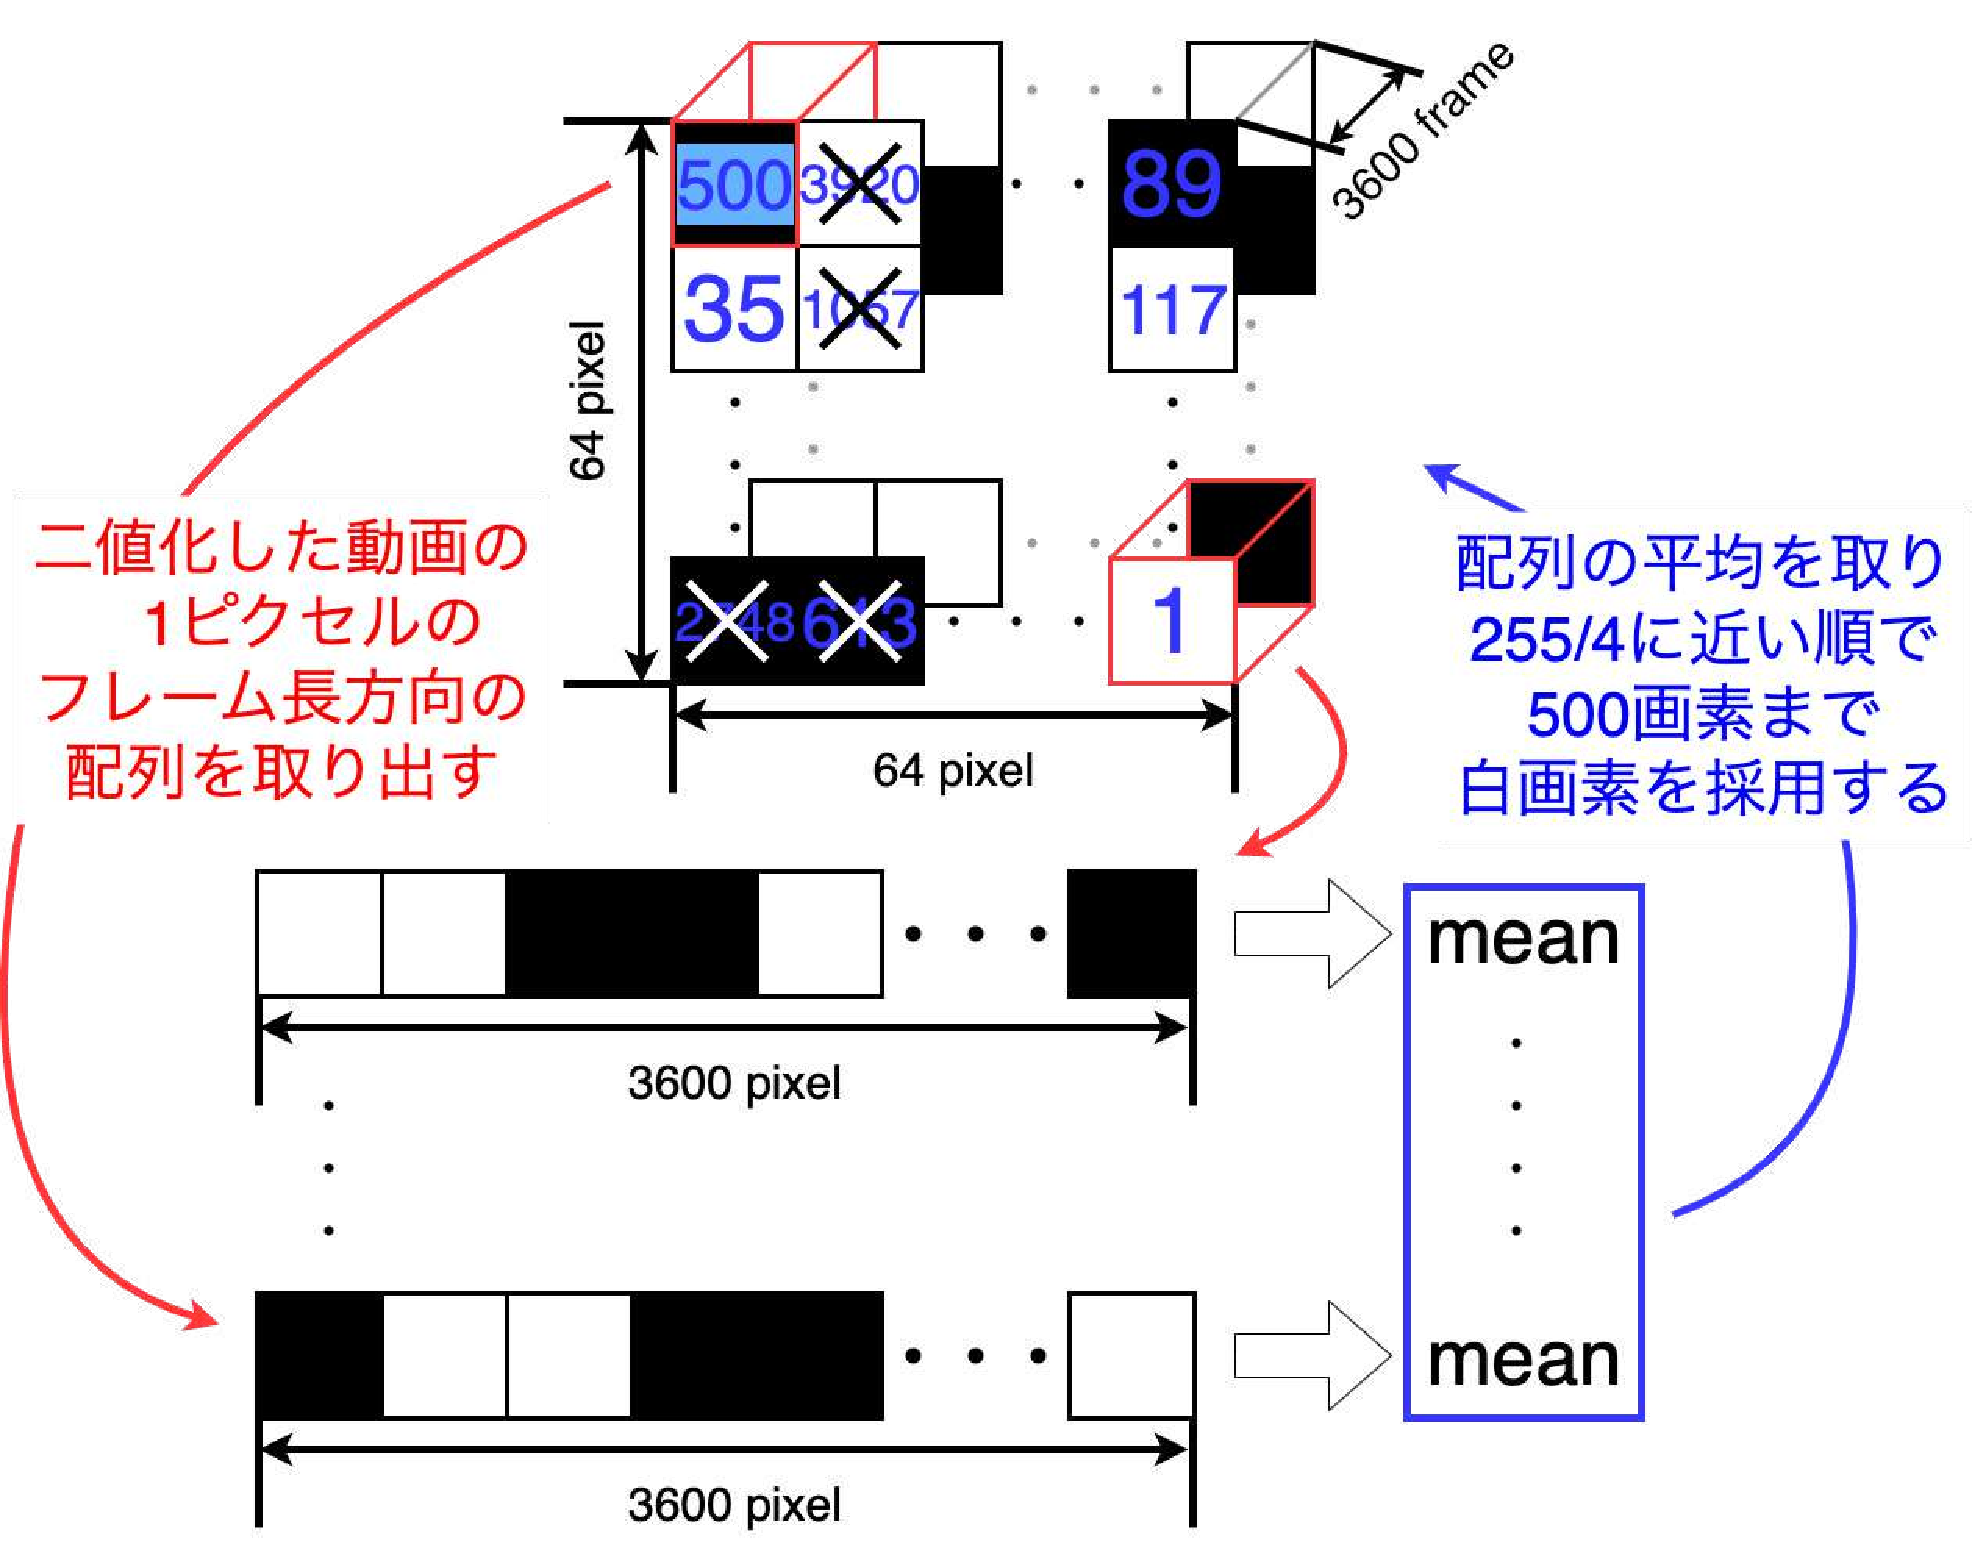
\includegraphics[width=120mm]{images/chart/choice.pdf}
  \end{center}
  \caption{白画素の制限方法}
  \label{choice}
\end{figure}

図\ref{choice}のように動画長の各ピクセルに注目する理由は,
対象の画素の変化量を知りたかったからである.
例えば手先が移動している場合,手先の元あった場所は背景色に変化するはずである.
逆に移動先では背景色が手先の色に変化する.
第1章,論文構成でも述べた通り,今回の研究では動作から優美さを抽出したいので,
動作の変化,動画データでは画素の変化を取り出したいと言い換えることができる.
そのために,1フレームごとの静止した画像ではなく,各ピクセル,動画長のデータを
用いることでデータを動作として扱うことができ,その平均を閾値で順序付けることで
目標とするに最も近い動作のみを抽出することができると考えた.

\subsection{ネットワーク構造}
編集した動画をそのまま使用するとフレーム数が多いので動画を複数に分割することを考えた.
図\ref{range}のように乱数を得た.乱数を視点として指定のフレーム長を切り取った.
それらをバッチ数まで集めた.乱数は各データ毎に個別に作成している.

動画群は結合して一つのデータとして扱うため,切り取る範囲が動画の繋ぎ目と被る可能性がある.
それを防ぐため,図\ref{decide_rand}のように予めそれぞれの動画長のフレームを
動画群から見た絶対数で保存しておく.指定した乱数がそれらの数値-指定フレームであった場合,
乱数を指定フレーム分追加することで再計算することなく固有の動画から指定範囲切り抜くことができる.

この手法は\cite{vivit}は着想を得た.ViViTでは動画を指定フレーム,指定ピクセルの
立方体で切り出し,Transformer Encoderにかけるという手法を取っている.
切り取った動画を検証するので動画全体を検証することはできないが,フレームを細かく分割することで
優美さ特定がより円滑に進むと考えた.

\begin{figure}[b]
  \begin{center}
    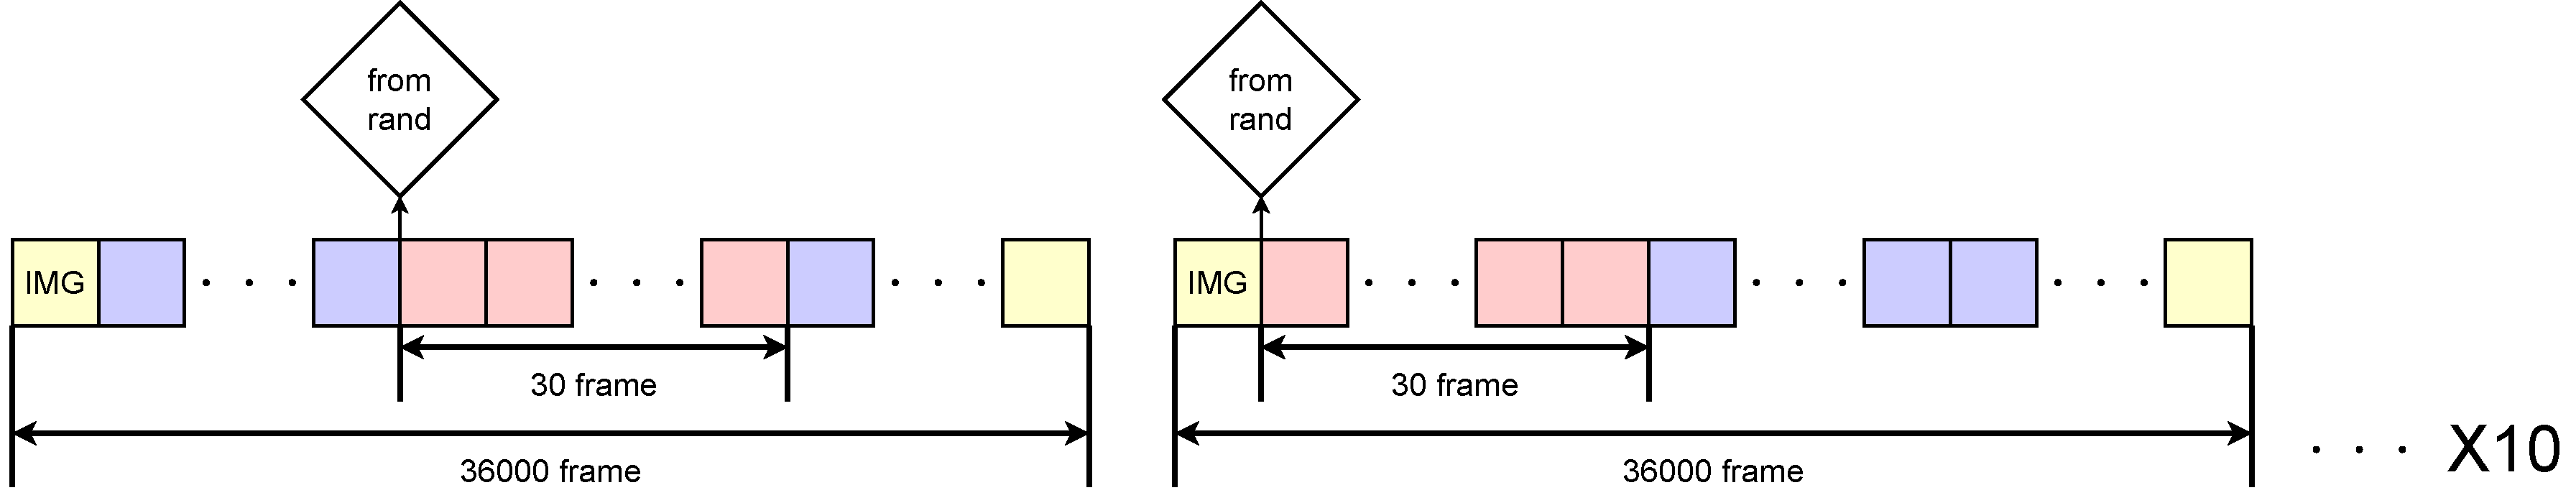
\includegraphics[width=120mm]{images/chart/range.pdf}
  \end{center}
  \caption{入力動画の分割方法}
  \label{range}
\end{figure}

\begin{figure}[b]
  \begin{center}
    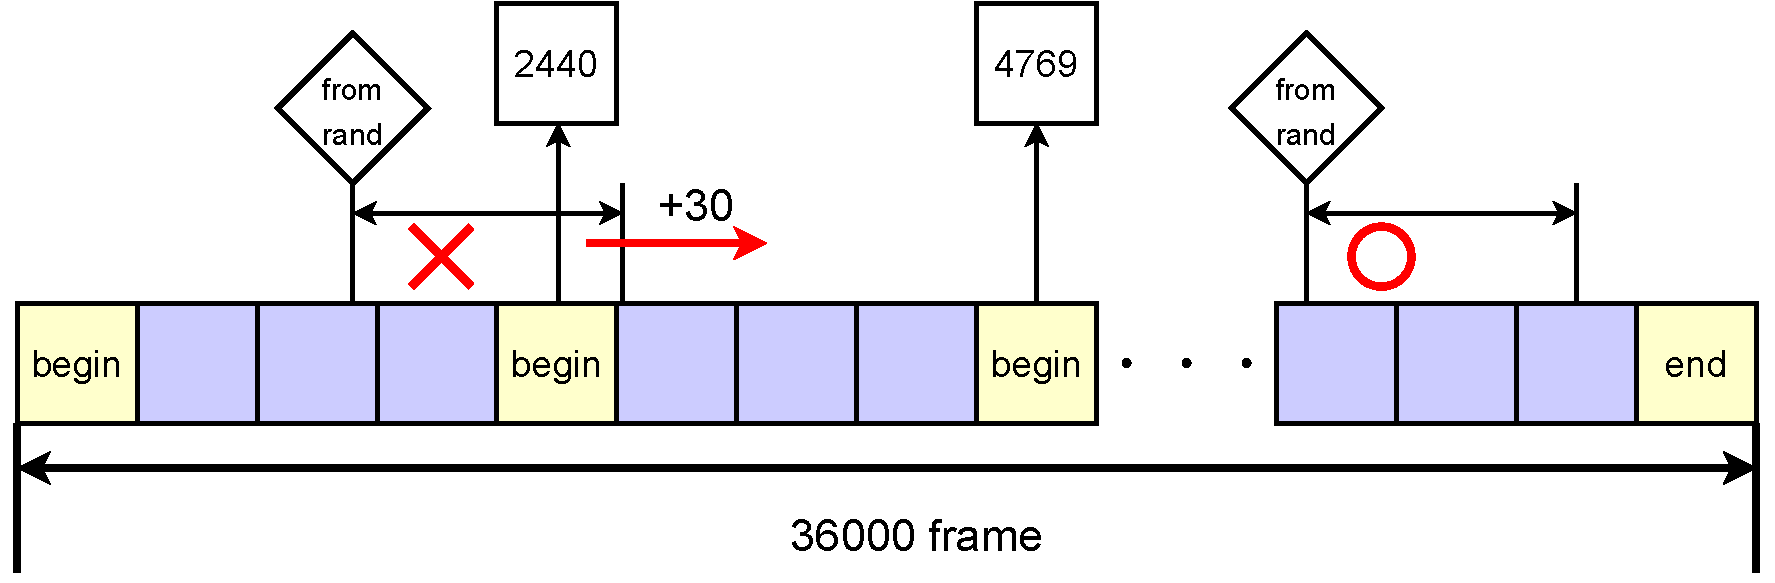
\includegraphics[width=120mm]{images/chart/decide_rand.pdf}
  \end{center}
  \caption{乱数の決定方法}
  \label{decide_rand}
\end{figure}
\clearpage

整形された動画データは二層の畳み込み層を通過する.
64×64の二次元データが128の一次元データに畳み込まれる.

次にピクセル情報を模した数値行列を同じ畳み込み層に通す.
この行列は64×64サイズに0から順にインデックス番号を持つ長さ指定フレーム長の行列である.
Transformerでは位置情報が喪失してしまうので位置情報を足し合わせることをする.
畳み込み後のデータは動画データではないのでインデックス番号を畳み込みすることで
同じ次元の位置情報を持たせることを試みた.

\begin{figure}[b]
  \begin{center}
    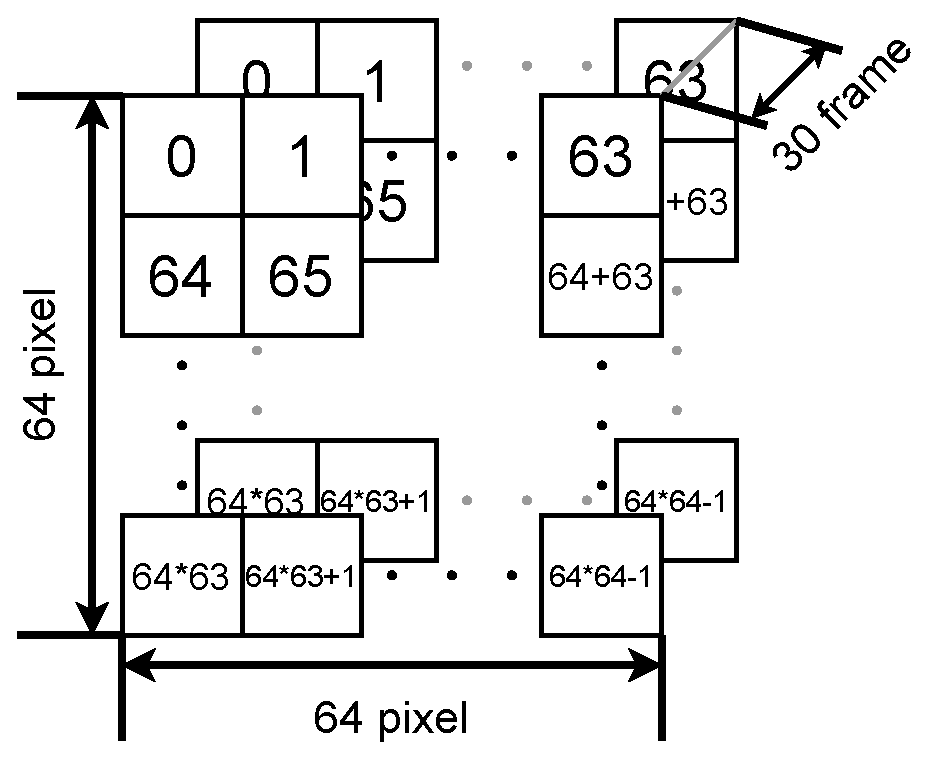
\includegraphics[width=120mm]{images/chart/embedding.pdf}
  \end{center}
  \caption{embeddingデータ}
  \label{embedding}
\end{figure}

加工された動画データと位置情報を足し合わせ,Transformer Encoderに通す.
ヘッドを二つに分割したレイヤーを二つ重ね合わせた.
これも\cite{vivit}に倣いこのような処理にした.実際,ヘッド数やレイヤー数は
これが最も精度良く推論できた.
\clearpage

最後に全結合層に通す.データを3に集約させるため,層を5つに分割し慎重に取り出した.
また,後半ではTanh(\ref{tanh})を活性化関数とすることでデータ全体が影響し合えるようにした.

\begin{equation}
  f(x) = \frac{e^x - e^{-x}}{e^x + e^{-x}}
  \label{tanh}
\end{equation}

ネットワーク全体をフローチャートにすると図\ref{flowchart}のようになる.

\begin{figure}[b]
  \begin{center}
    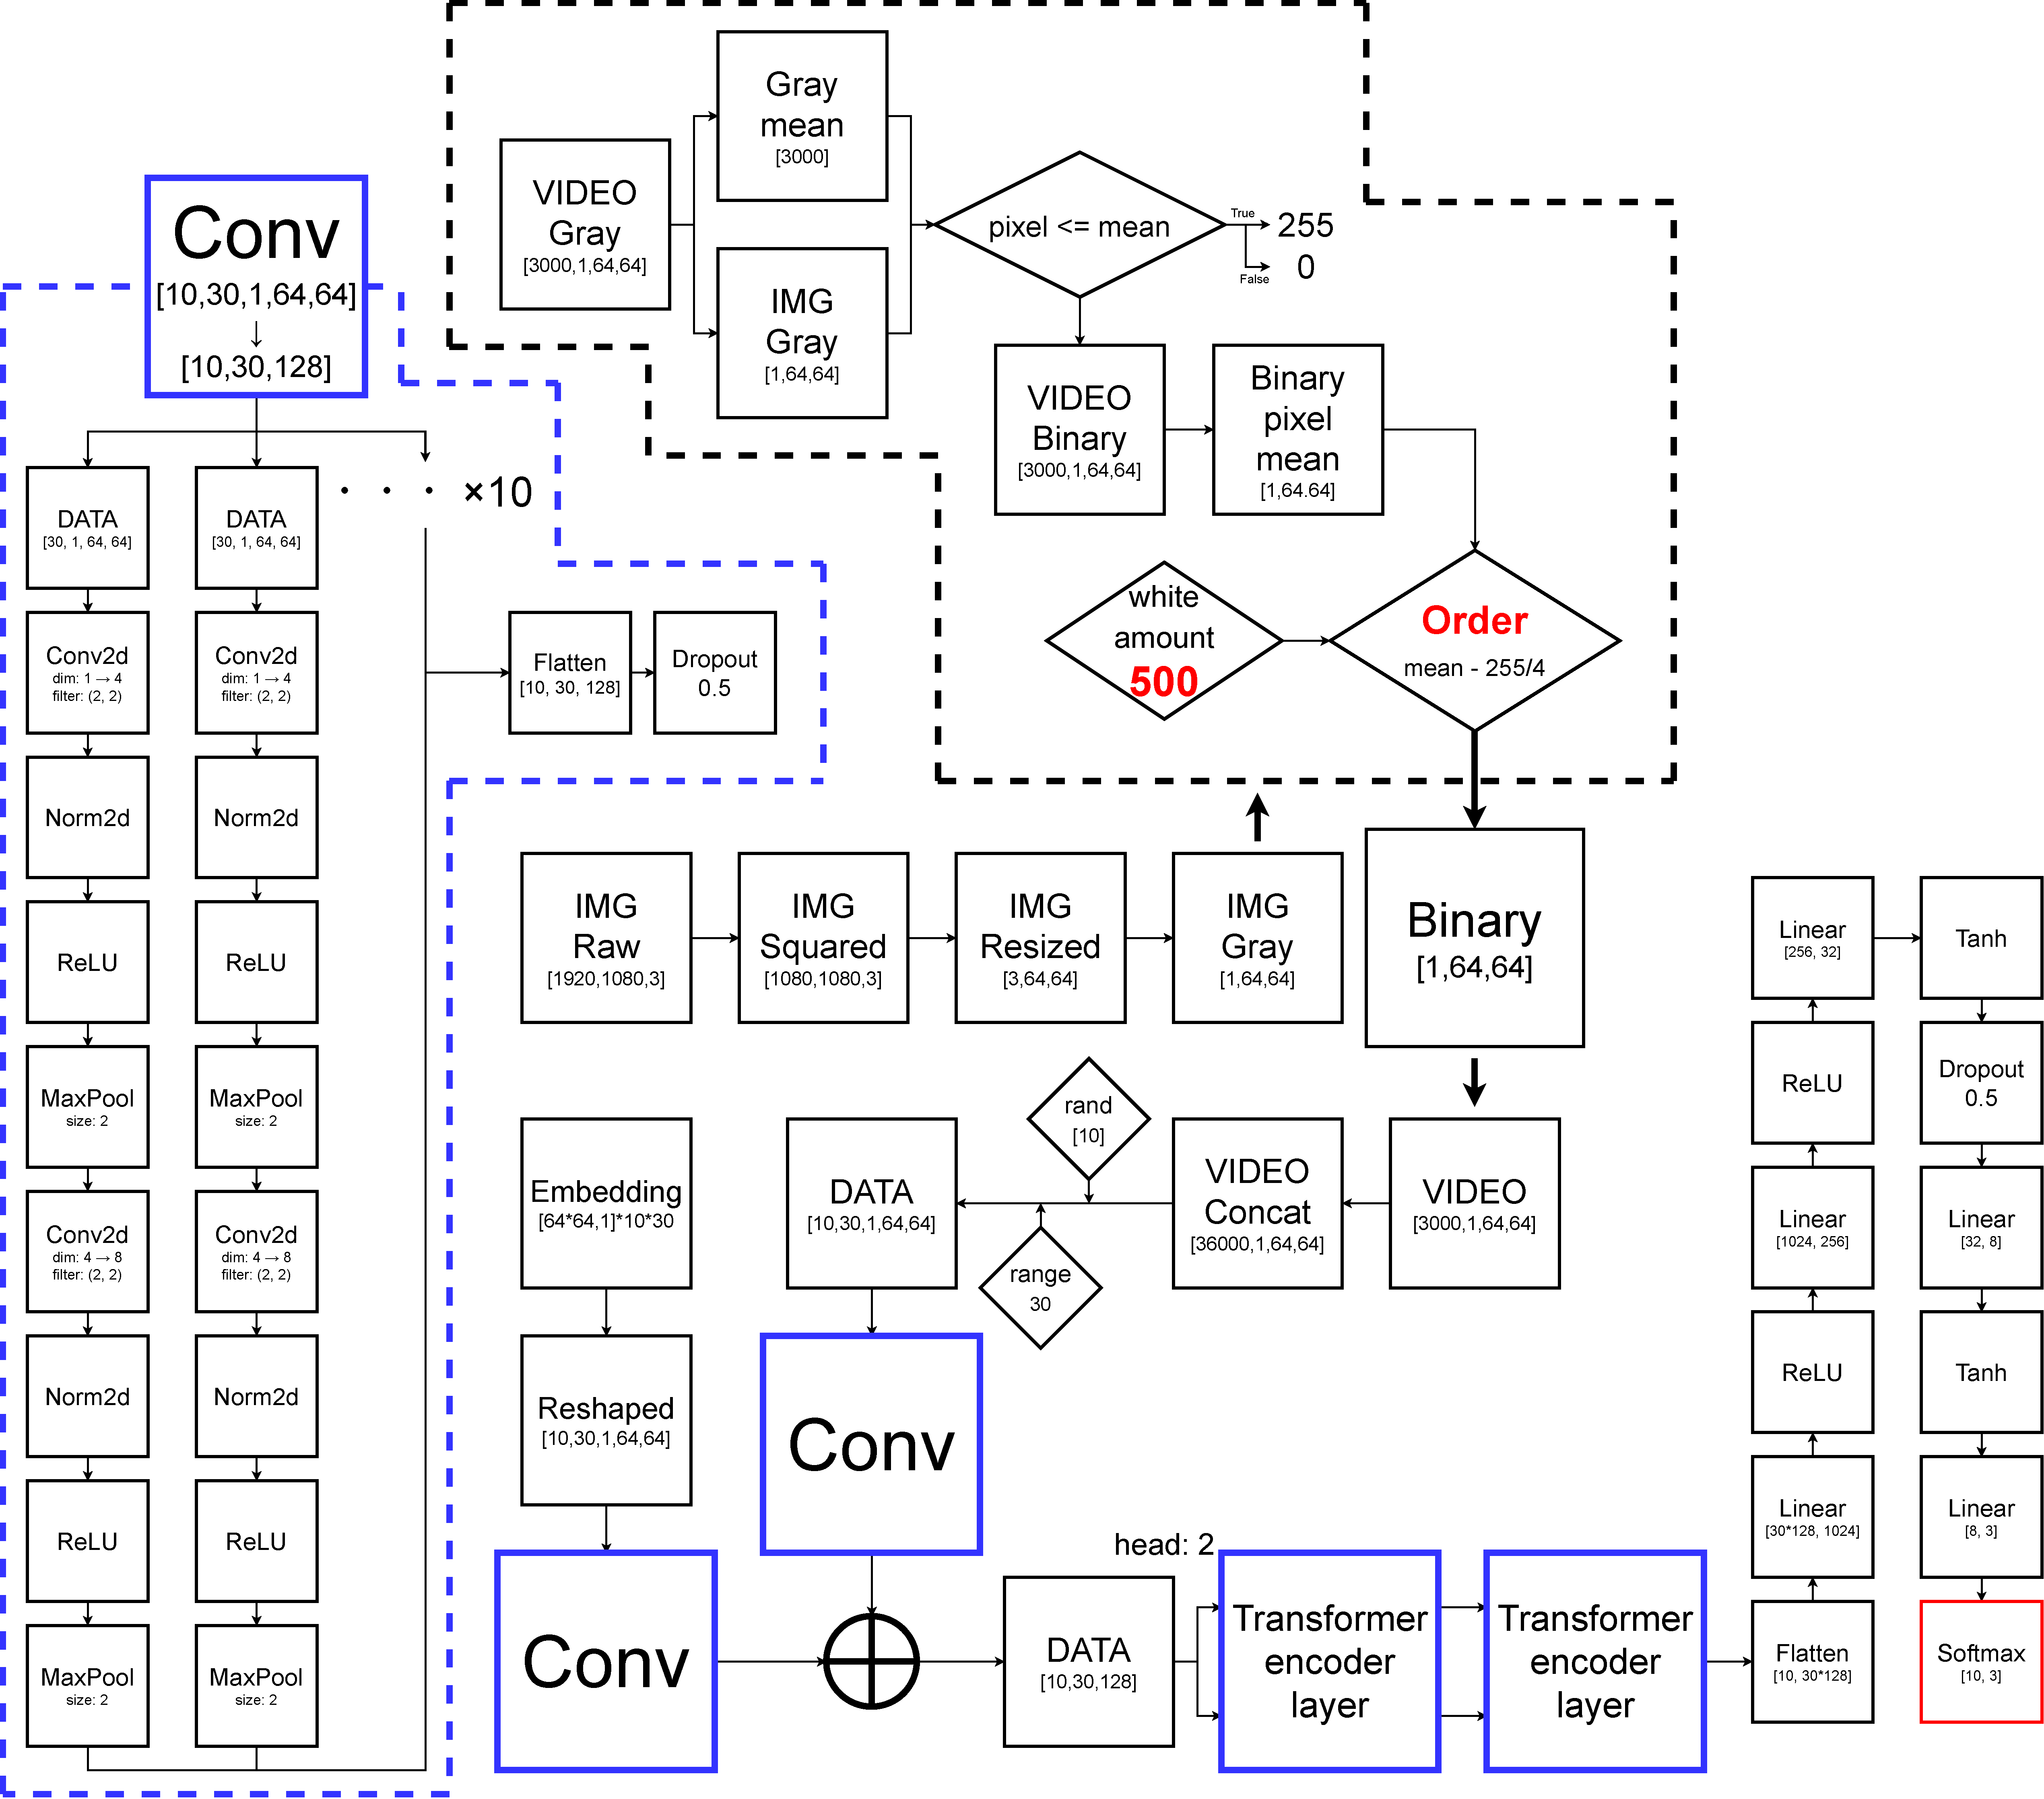
\includegraphics[width=120mm]{images/chart/flowchart.pdf}
  \end{center}
  \caption{ネットワーク全体}
  \label{flowchart}
\end{figure}
\clearpage

\subsection{精度}
作成したネットワークが学習できているか確認するために,動画数を変化させて
その精度の推移を確認した.
表\ref{result}のように動画を3つずつ増やした結果,精度が向上していることがわかった.

\begin{table}[b]
  \centering
  \begin{tabular}{|c|} \hline
    結果と使用動画 \\ \hline
    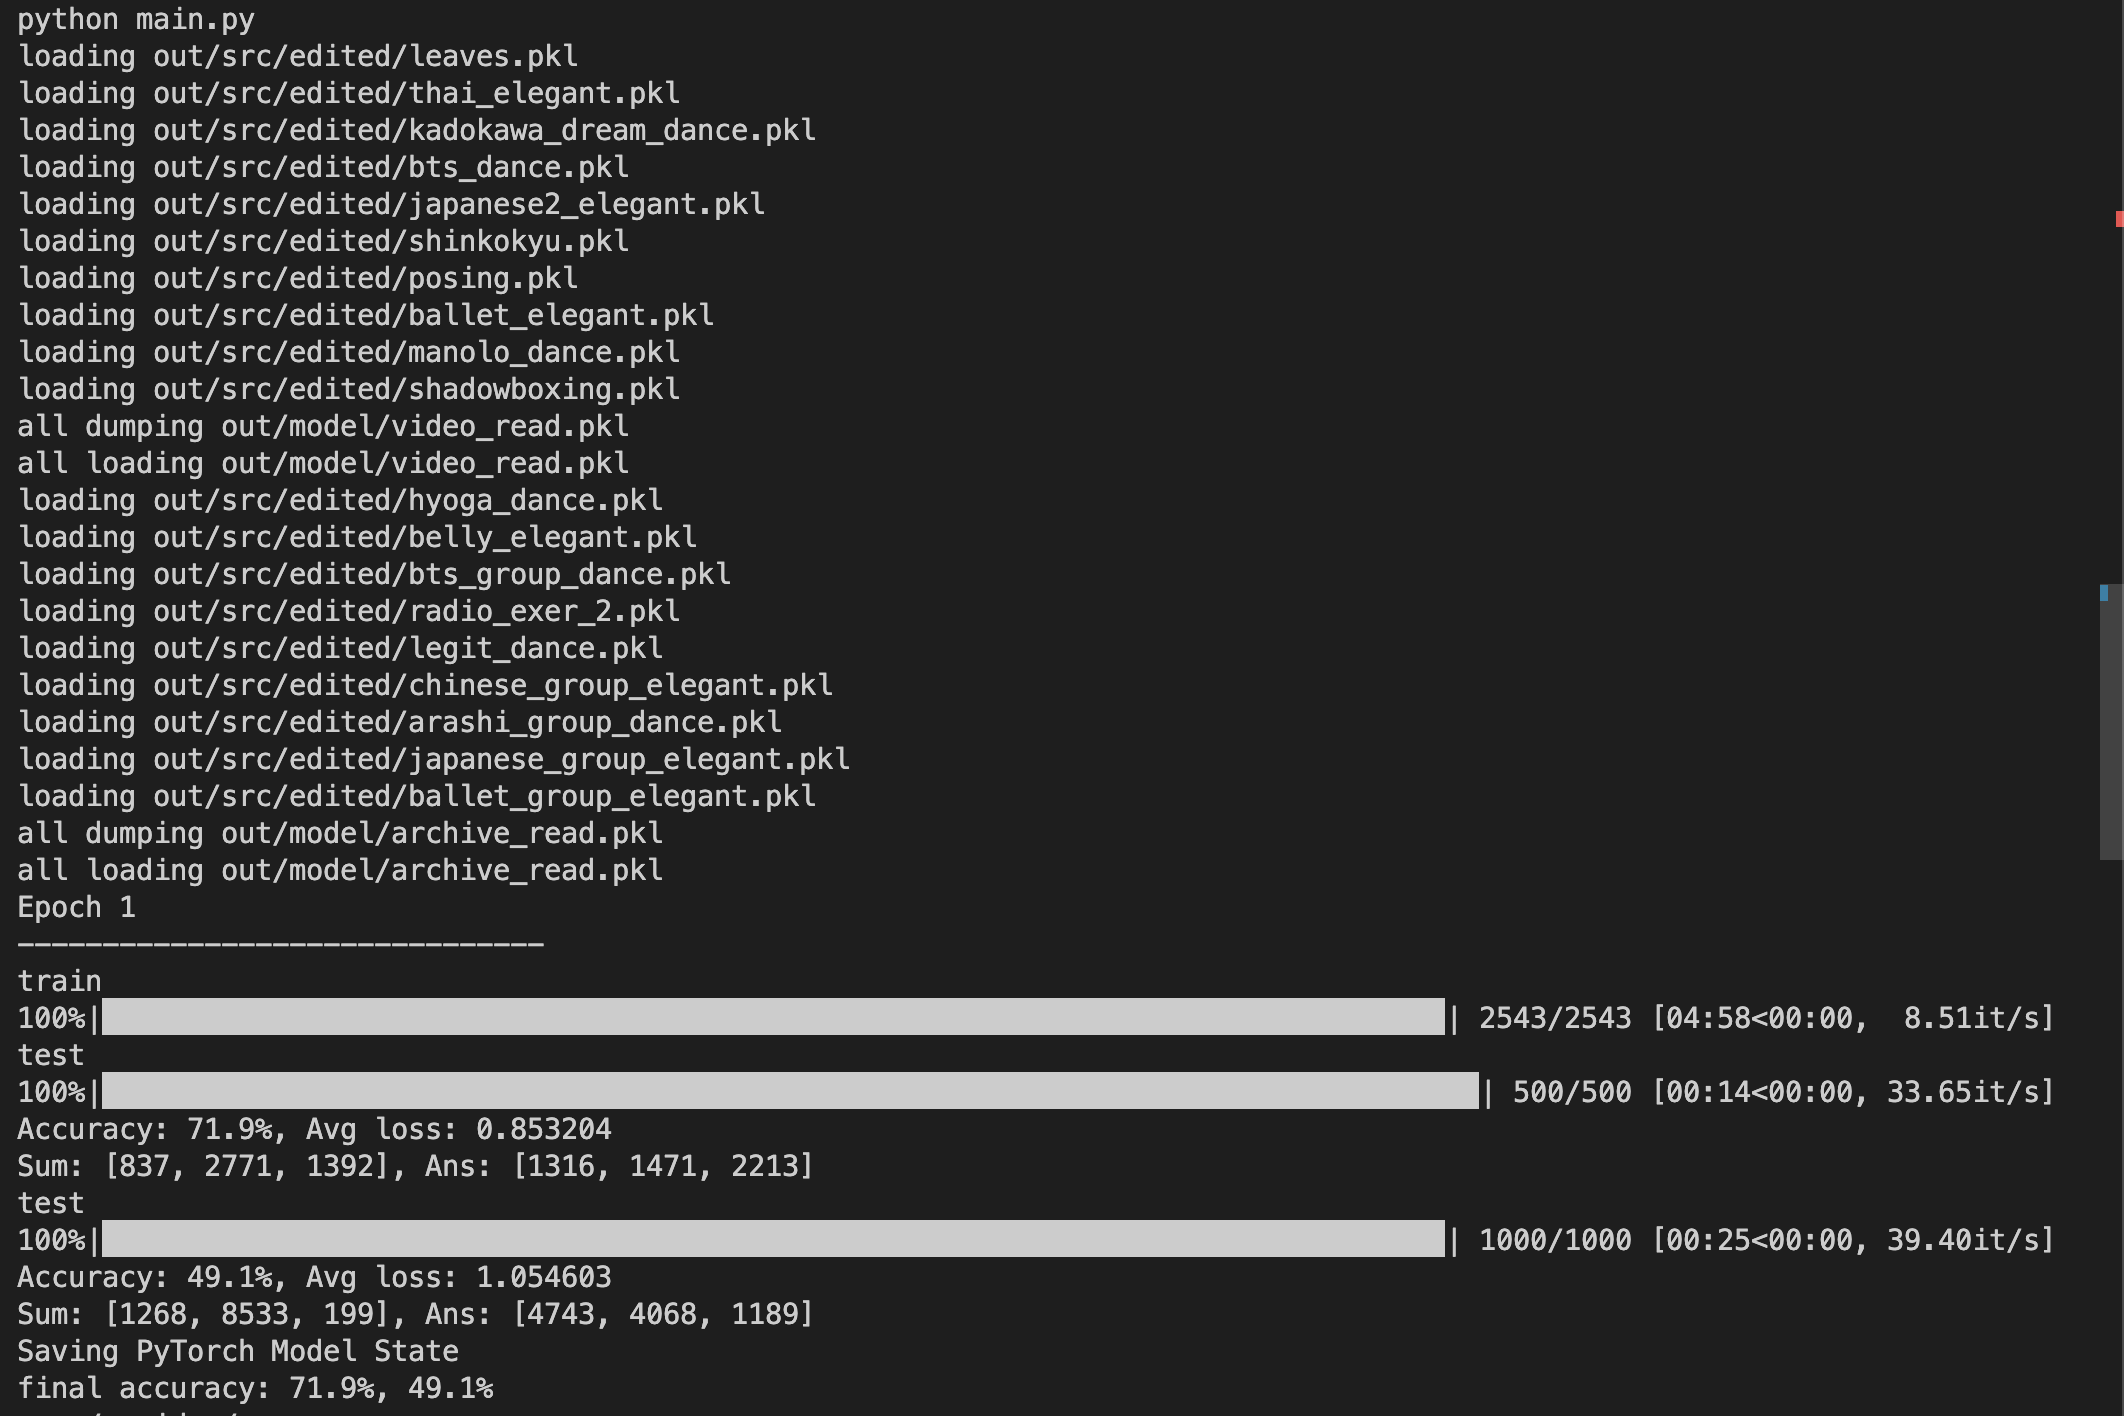
\includegraphics[width=120mm]{images/net_result/result10.png}
    \\
    \cite{ballet}\cite{thai}\cite{jpn2}
    \cite{kadokawa}\cite{bts}\cite{manolo}
    \cite{posing}\cite{boxing}\cite{shinkokyu}\cite{leaves}
    \\ \hline
    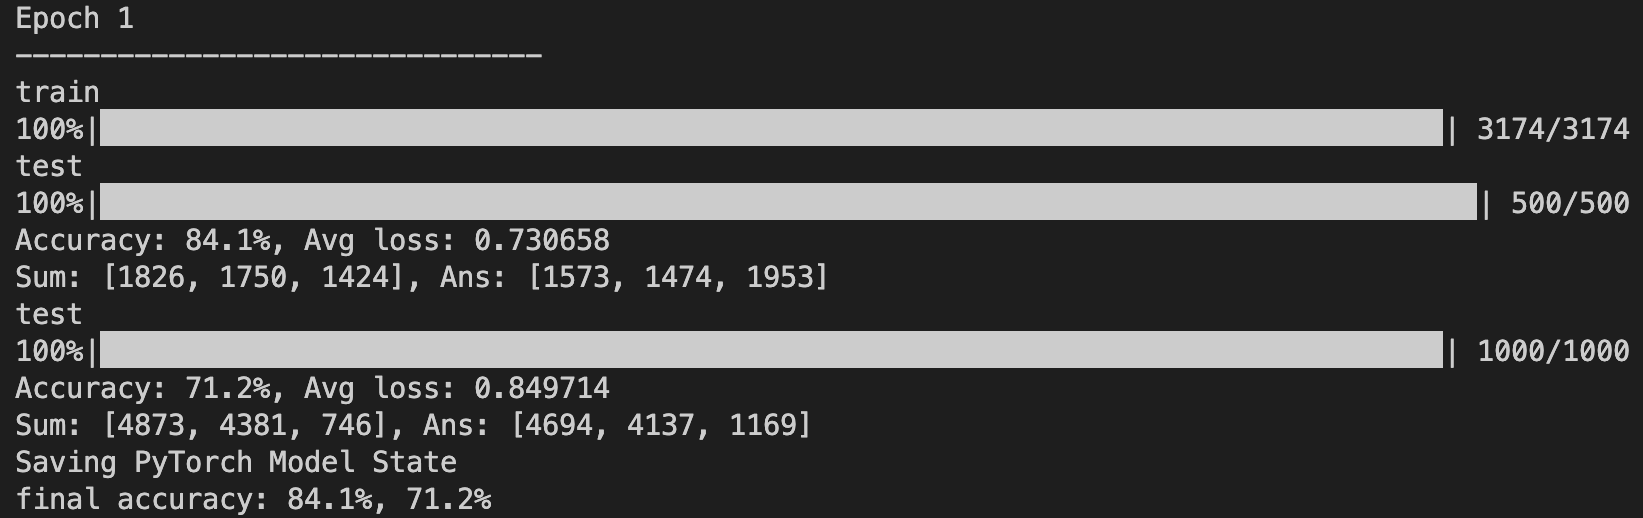
\includegraphics[width=120mm]{images/net_result/result13.png}
    \\
    \cite{jpn}\cite{ballet}\cite{thai}\cite{jpn2}
    \cite{ariana}\cite{kadokawa}\cite{bts}\cite{manolo}
    \cite{posing}\cite{boxing}\cite{running}\cite{shinkokyu}\cite{leaves}
    \\ \hline
    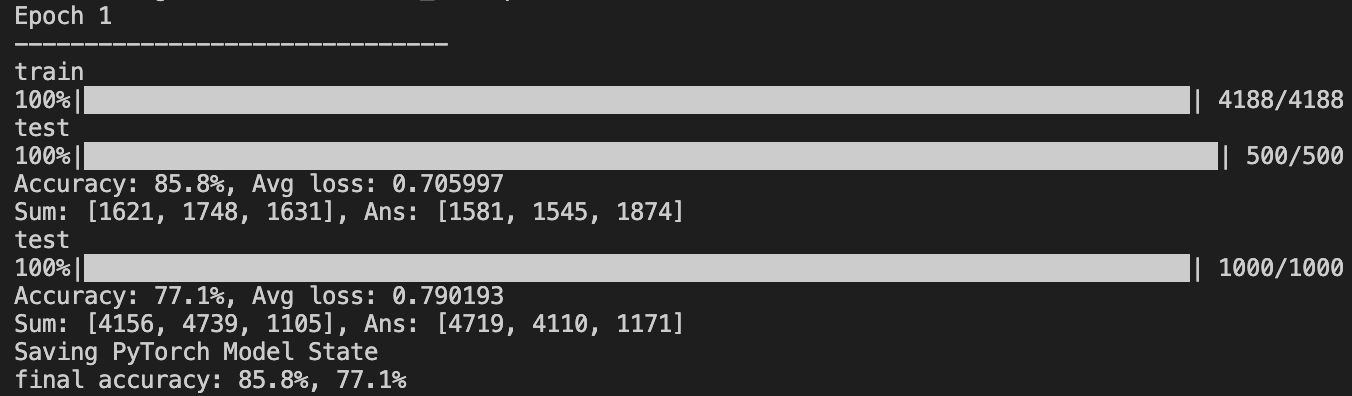
\includegraphics[width=120mm]{images/net_result/result16.png}
    \\
    \cite{jpn}\cite{china}\cite{ballet}\cite{thai}\cite{jpn2}
    \cite{ariana}\cite{kadokawa}\cite{bts}\cite{manolo}\cite{aito}
    \cite{radio}\cite{posing}\cite{boxing}\cite{running}\cite{shinkokyu}\cite{leaves}
    \\ \hline
  \end{tabular}
  \caption{使用動画別の精度}
  \label{result}
\end{table}
\clearpage

次にバッチサイズ別に精度の推移を確認した.バッチとは,データをひとまとめにして同時に学習させることである.
表\ref{batch}のようにbatchが少ない方が学習データは精度良く学習できるが,推論時には10辺りが
精度良く学習できることが分かった.

バッチサイズを大きくするとそれぞれの層のデータも大きくなるので学習に対してはバッチサイズは小さな方が精度が出る.
一方推論時には層のデータが小さいと対応できない場面に多々出くわすので,バッチサイズは10程度が基準となっている.

\begin{table}[b]
  \centering
  \begin{tabular}{|c|} \hline
    結果とバッチサイズ \\ \hline
    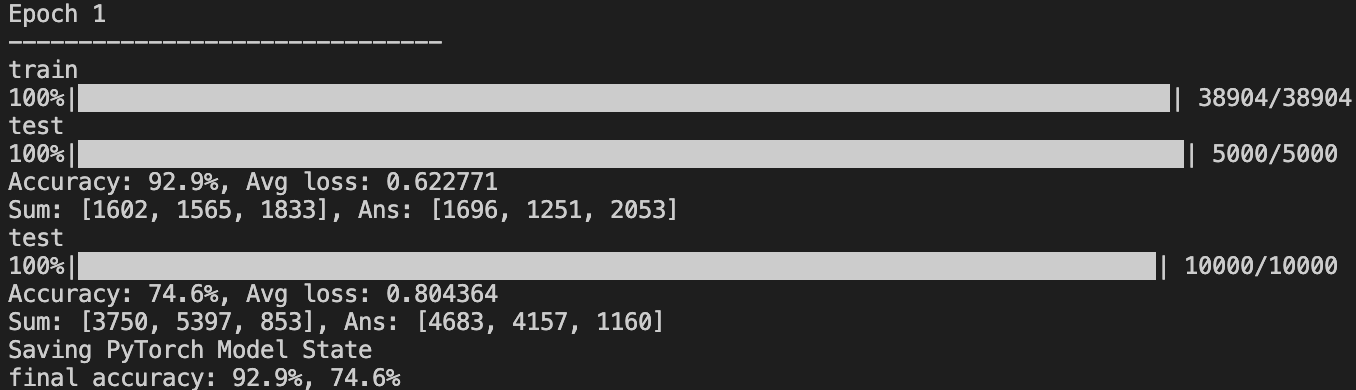
\includegraphics[width=120mm]{images/net_result/batch1.png}
    \\ 1 \\ \hline
    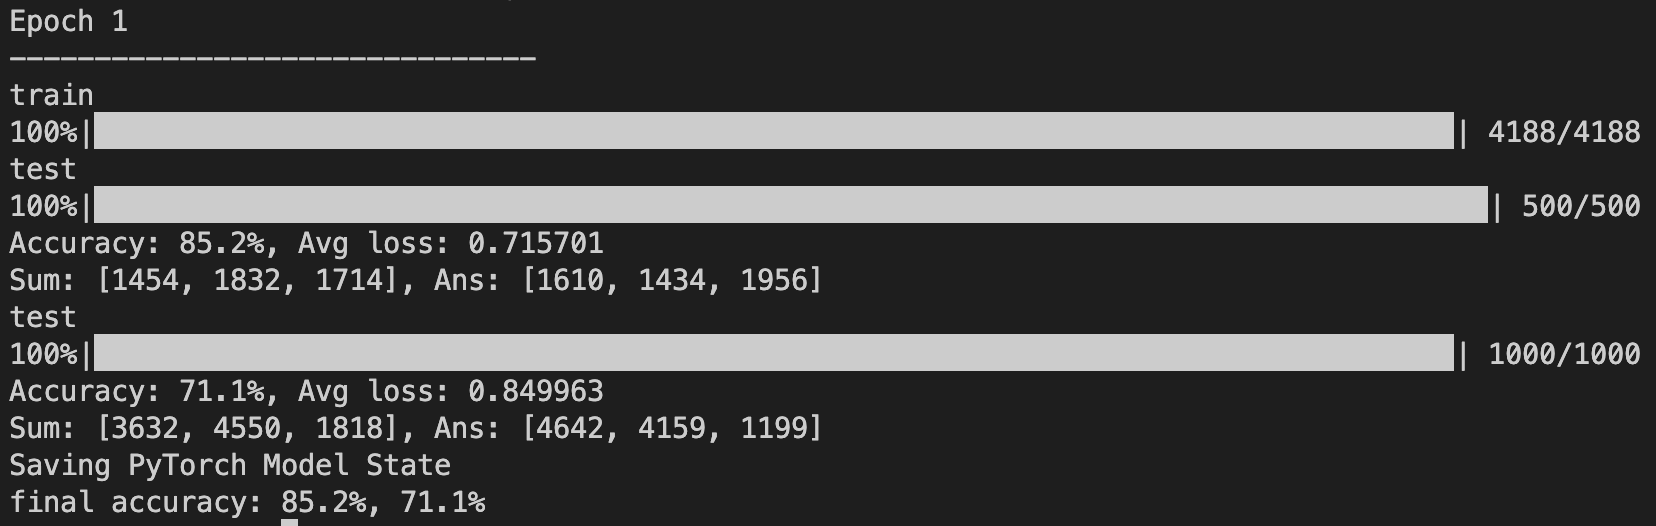
\includegraphics[width=120mm]{images/net_result/batch10.png}
    \\ 10 \\ \hline
    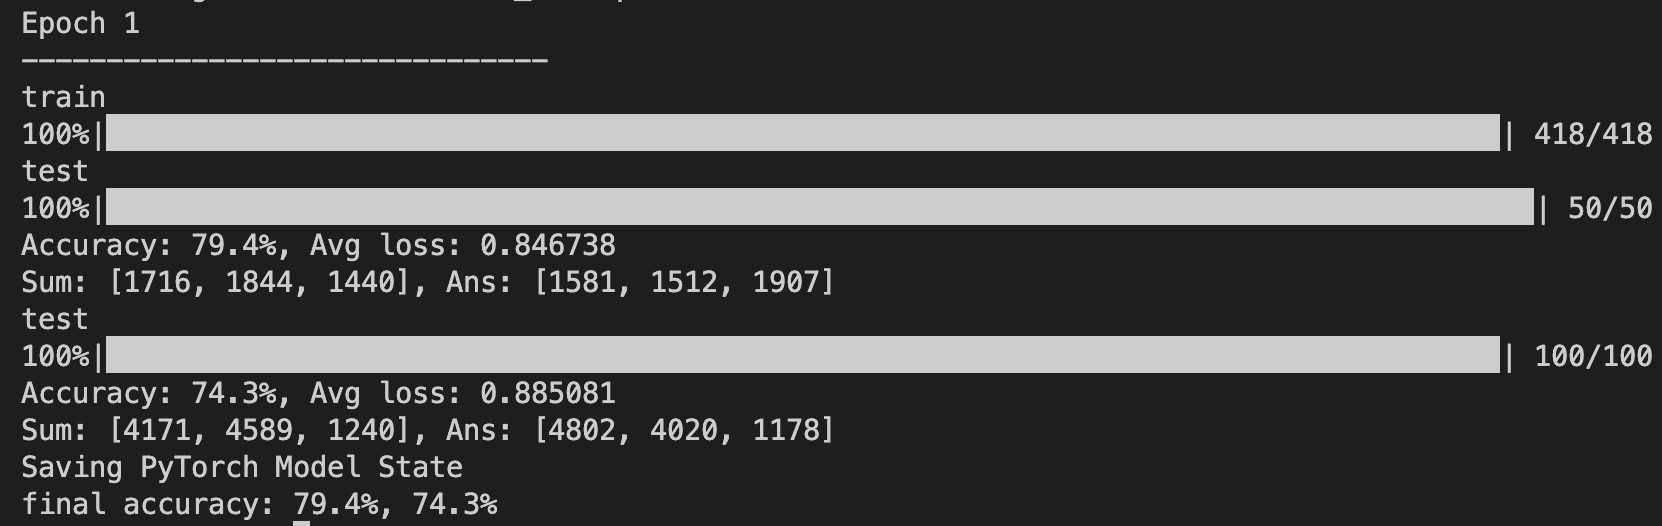
\includegraphics[width=120mm]{images/net_result/batch100.png}
    \\ 100 \\ \hline
  \end{tabular}
  \caption{batch別の精度}
  \label{batch}
\end{table}
\clearpage

今回の実験でバッチサイズ10が効率よく検証できる結果となったので判断根拠可視化でもこれを採用することとした.

次に学習,エポック毎で損失がどのように推移するか確認した.エポックとは,同一のデータを
繰り返し学習させることである.
表\ref{epoch}のように1回目のエポックでほとんど収束して行き,エポックを重ねるごとに
その値の揺れが小さくなっていることが分かった.

これらのことから制作したネットワークが正常に学習を進めていることが分かった.
また,学習データに対して8割程度の精度であったとしても,推論時も7.5割程度で
判別することができることが分かった.

\begin{table}[b]
  \centering
  \begin{tabular}{|c|} \hline
    結果とエポック数 \\ \hline
    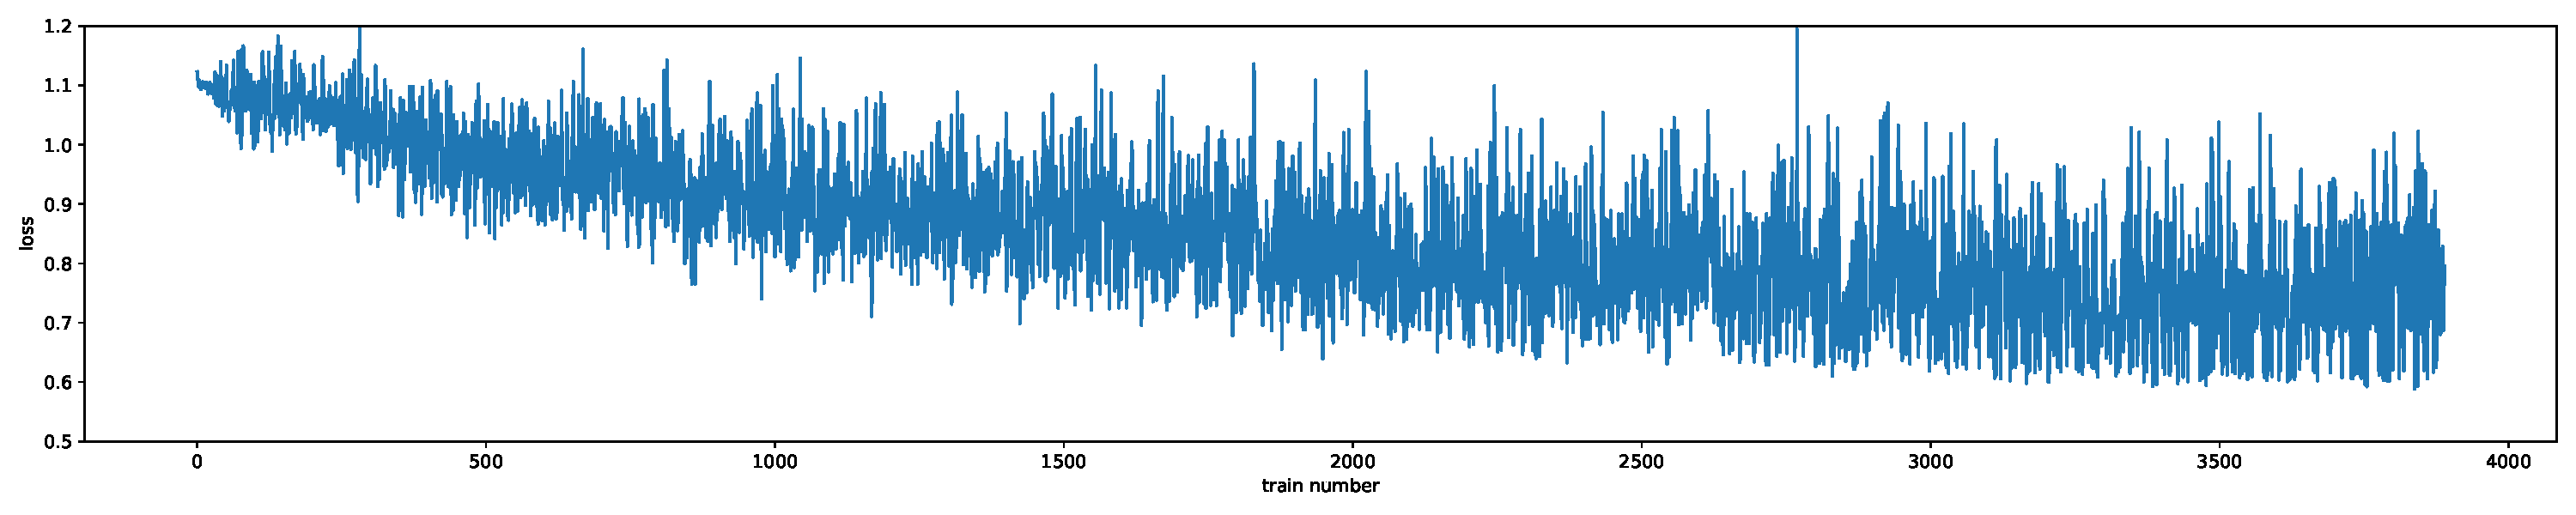
\includegraphics[width=130mm]{images/net_result/epoch_1.pdf}
    \\ 1 \\ \hline
    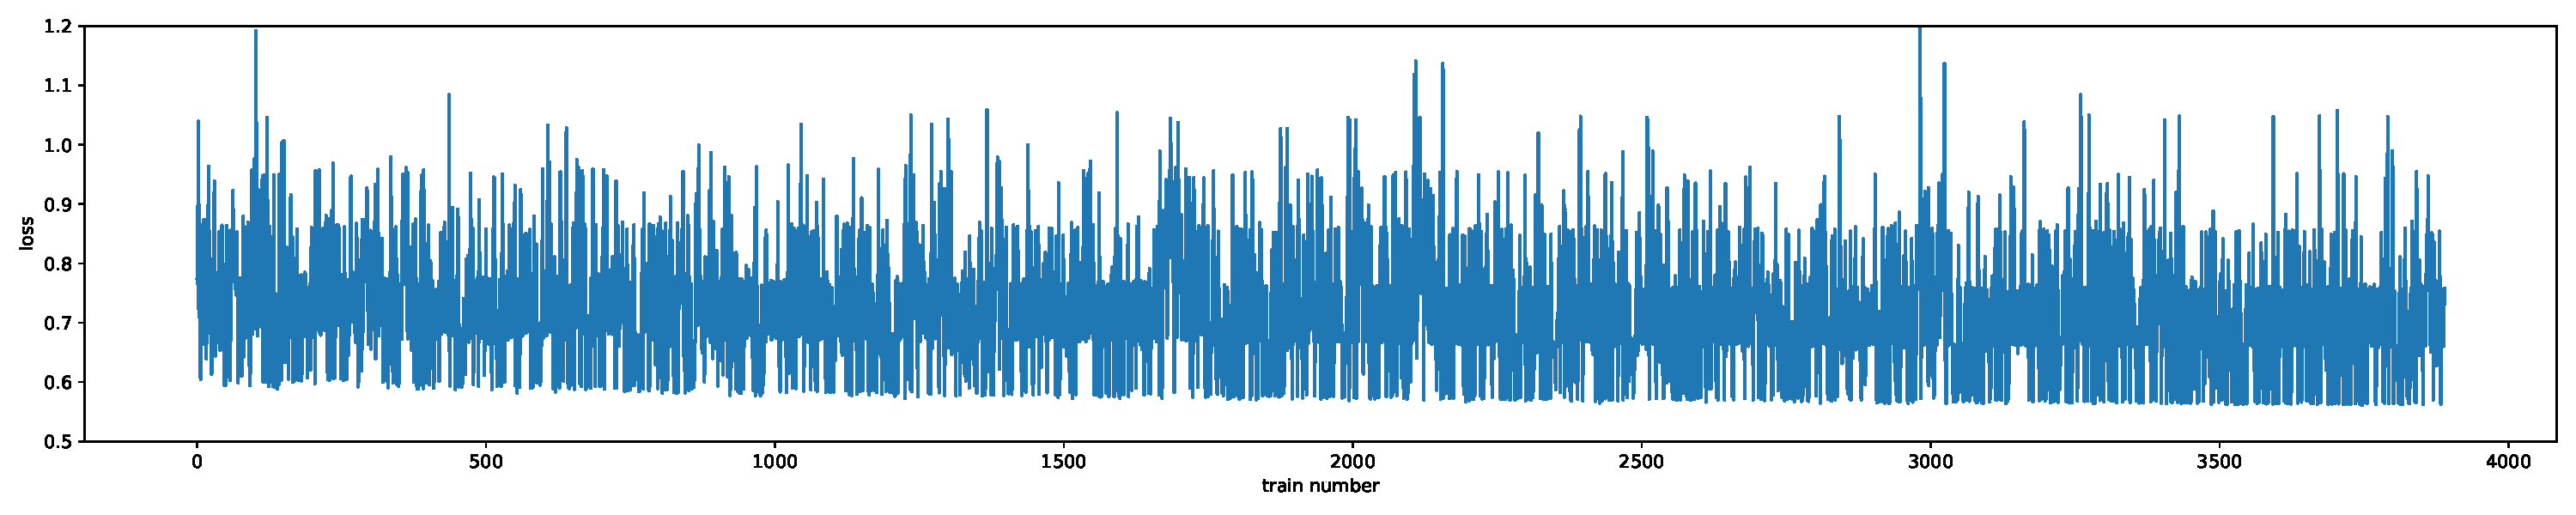
\includegraphics[width=130mm]{images/net_result/epoch_2.pdf}
    \\ 2 \\ \hline
    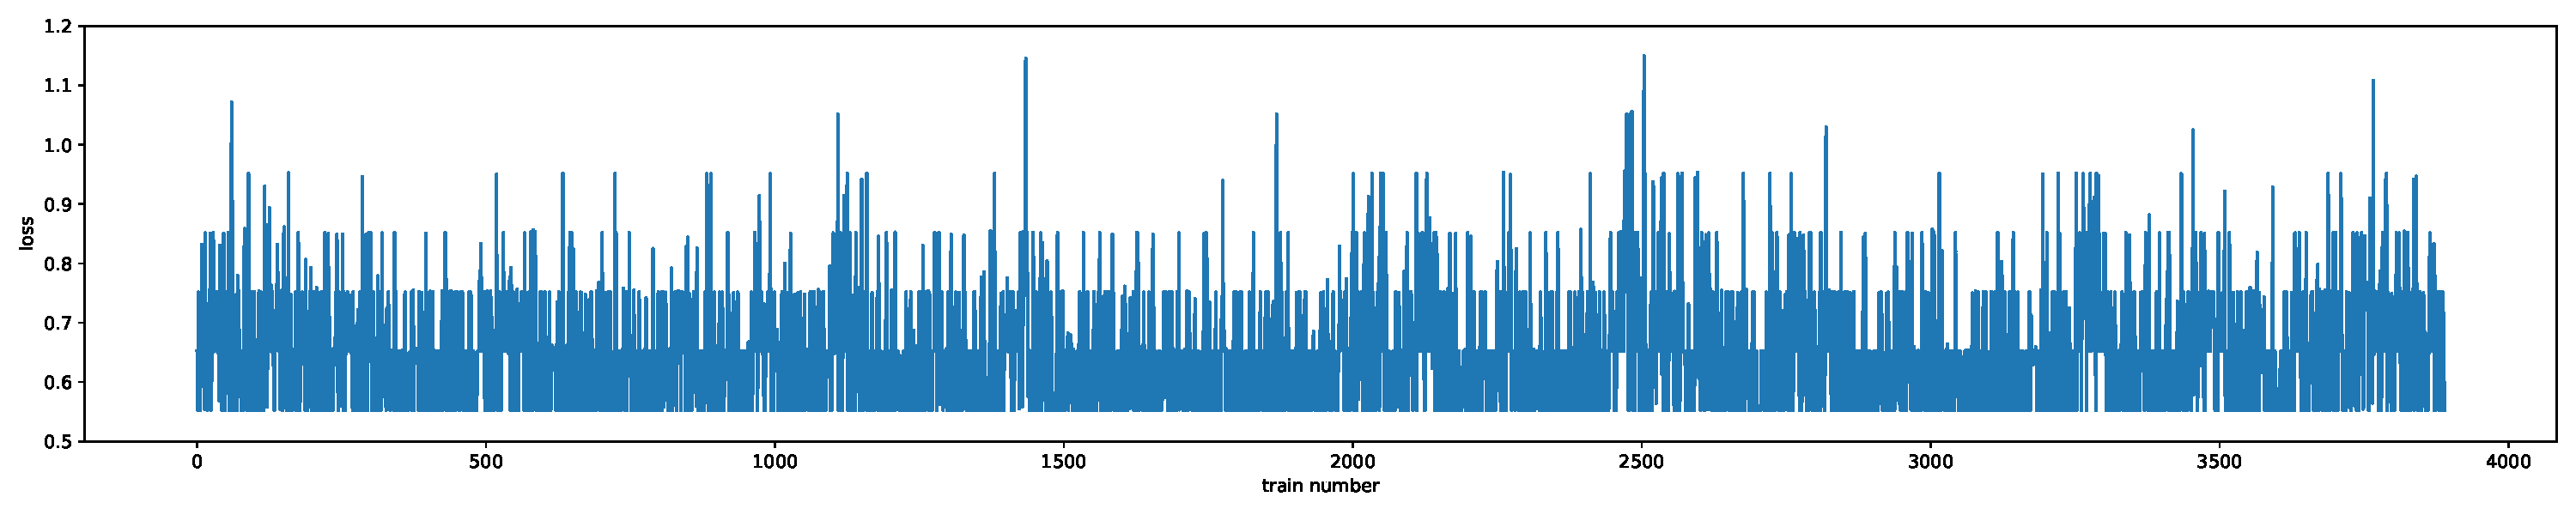
\includegraphics[width=130mm]{images/net_result/epoch_10.pdf}
    \\ 10 \\ \hline
  \end{tabular}
  \caption{epoch毎の損失推移}
  \label{epoch}
\end{table}
\clearpage